\documentclass[a4 paper]{article}
% Set target color model to RGB
\usepackage[inner=2.0cm,outer=2.0cm,top=2.5cm,bottom=2.5cm]{geometry}
\usepackage{setspace}
\usepackage[rgb]{xcolor}
\definecolor{codegreen}{rgb}{0,0.6,0}
\definecolor{codegray}{rgb}{0.5,0.5,0.5}
\definecolor{codepurple}{rgb}{0.58,0,0.82}
\definecolor{backcolour}{rgb}{0.95,0.95,0.92}
\usepackage{verbatim}
\usepackage[]{algorithm2e}
\usepackage{subcaption}
\usepackage{amsgen,amsmath,amstext,amsbsy,amsopn,amssymb}
\usepackage{fancyhdr}
\usepackage{listings}
\lstdefinestyle{mystyle}{
    backgroundcolor=\color{backcolour},   
    commentstyle=\color{codegreen},
    keywordstyle=\color{magenta},
    numberstyle=\tiny\color{codegray},
    stringstyle=\color{codepurple},
    basicstyle=\ttfamily\footnotesize,
    breakatwhitespace=false,         
    breaklines=true,                 
    captionpos=b,                    
    keepspaces=true,                 
    numbers=left,                    
    numbersep=2pt,                  
    showspaces=false,                
    showstringspaces=false,
    showtabs=false,                  
    tabsize=2
}

\lstset{style=mystyle}
\usepackage[natbibapa]{apacite} 
\usepackage[colorlinks=true, urlcolor=blue, linkcolor=blue, citecolor=blue]{hyperref}
\usepackage[colorinlistoftodos]{todonotes}
\usepackage{rotating}
%\usetikzlibrary{through,backgrounds}
\hypersetup{%
pdfauthor={Ashudeep Singh},%
pdftitle={Homework},%
pdfkeywords={Tikz,latex,bootstrap,uncertaintes},%
pdfcreator={PDFLaTeX},%
pdfproducer={PDFLaTeX},%
}
%\usetikzlibrary{shadows}
% \usepackage[francais]{babel}
\usepackage{booktabs}
\newcommand{\ra}[1]{\renewcommand{\arraystretch}{#1}}

\newtheorem{thm}{Theorem}[section]
\newtheorem{prop}[thm]{Proposition}
\newtheorem{lem}[thm]{Lemma}
\newtheorem{cor}[thm]{Corollary}
\newtheorem{defn}[thm]{Definition}
\newtheorem{rem}[thm]{Remark}
\numberwithin{equation}{section}

\newcommand{\homework}[6]{
   \pagestyle{myheadings}
   \thispagestyle{plain}
   \newpage
   \setcounter{page}{1}
   \noindent
   \begin{center}
   \framebox{
      \vbox{\vspace{2mm}
    \hbox to 6.28in { {\bf Deep Learning 2020 \hfill {\small (#2)}} }
       \vspace{6mm}
       \hbox to 6.28in { {\Large \hfill #1  \hfill} }
       \vspace{6mm}
       \hbox to 6.28in { {\it Instructor: {\rm #3} \hfill Name: {\rm #5}, Netid: {\rm #6}} }
       %\hbox to 6.28in { {\it TA: #4  \hfill #6}}
      \vspace{2mm}}
   }
   \end{center}
   \markboth{#5 -- #1}{#5 -- #1}
   \vspace*{4mm}
}

\newcommand{\problem}[2]{~\\\fbox{\textbf{Problem #1}}\hfill (#2 points)\newline\newline}
\newcommand{\subproblem}[1]{~\newline\textbf{(#1)}}
\newcommand{\D}{\mathcal{D}}
\newcommand{\Hy}{\mathcal{H}}
\newcommand{\VS}{\textrm{VS}}
\newcommand{\solution}{~\newline\textbf{\textit{(Solution)}} }

\newcommand{\bbF}{\mathbb{F}}
\newcommand{\bbX}{\mathbb{X}}
\newcommand{\bI}{\mathbf{I}}
\newcommand{\bX}{\mathbf{X}}
\newcommand{\bY}{\mathbf{Y}}
\newcommand{\bepsilon}{\boldsymbol{\epsilon}}
\newcommand{\balpha}{\boldsymbol{\alpha}}
\newcommand{\bbeta}{\boldsymbol{\beta}}
\newcommand{\0}{\mathbf{0}}

% Changelog
% 26 Oct. First version
% 30 Oct. Removed page length indicators. Added appendix, question section and some extra explanations.
%

% BEGIN DOCUMENT
\begin{document}
\homework{Submission Assignment \#2}{Due: 18 Nov 2020}{Jakub Tomczak}{}{Asif Anwar}{aar216}

The following section layout is a suggestion for the structure of the report. If it doesn't quite fit, you can use whatever structure does work.

\section{Question answers}
\paragraph{Question 1} \textit{Derivation of $\frac{X}{Y}$ where X and Y are two metrics in respect to X and Y are shown below.}
\begin{itemize}
    \item $\frac{\delta}{\delta X} \delta(\frac{X}{Y}) = \sum_{kl} \frac{\delta(\frac{X_{kl}}{Y_{kl}})}{\delta X_{ij}} = \frac{1}{Y_{ij}}$
    \item $\frac{\delta}{\delta Y} \delta(\frac{X}{Y}) = \sum_{kl} \frac{\delta(\frac{X_{kl}}{Y_{kl}})}{\delta Y_{ij}} = - \frac{X_{ij}}{Y_{ij}^2}$
\end{itemize}
\textit{The backward of X and Y for element wise division will be as derived above $\frac{1}{Y_ij}$, $\frac{X_ij}{Y_{ij}^2}$}
\paragraph{Note:} \textit{Considering backward function requires the comparison with loss and question 2 has the similar requirements, the full backward inrespect to loss is shown in question 2. }
\paragraph{Question 2} \textit{Let's consider the function \emph{f} has been applied to the given computational graph and \emph{l} is the loss of the function. And its given that derivative of \emph{f} if \emph{f'}. If we calculate the derivatives we get below:}
\begin{itemize}
    \item $X_{ij}^\nabla = \frac{\delta l}{\delta X_{ij}} = \sum \frac{\delta l}{\delta f} \frac{\delta f}{X_{ij}} = \sum_{kl} f_{kl}^\nabla \frac{\delta(\frac{X_{kl}}{Y_{kl}})}{\delta X_{ij}} =  f_{ij}^\nabla  \sum_{kl} \frac{\delta(\frac{X_{kl}}{Y_{kl}})}{\delta X_{ij}} = f_{ij}^\nabla \frac{1}{Y_{ij}} $
    \item $Y_{ij}^\nabla = \frac{\delta l}{\delta Y_{ij}} = \sum \frac{\delta l}{\delta f} \frac{\delta f}{Y_{ij}} = \sum_{kl} f_{kl}^\nabla \frac{\delta(\frac{X_{kl}}{Y_{kl}})}{\delta Y_{ij}} =  f_{ij}^\nabla  \sum_{kl} \frac{\delta(\frac{X_{kl}}{Y_{kl}})}{\delta Y_{ij}} = f_{ij}^\nabla \frac{X_{ij}}{Y_{ij}^2}$ 
\end{itemize}
\textit{From above equations we can see that backward of F is the element-wise application of f' applied to the elements of X, multiplied by the gradient of the loss with respect to the outputs.}
\paragraph{Question 3} \textit{Given, \textbf matrix {W} is the weights and matrix \textit{X} is the batch input where n is number of instance and f is number features. For this we can do matrix dot product or matrix multiplication to get the \emph{output} of the node. The derivation of this multiplication operation is shown below.}\\
\textit{Forward $W \cdot X^T$}\\
\textit{Backward:}
\begin{itemize}
    \item $X^\delta = \frac{\delta l}{\delta X} = \sum \frac{\delta l}{\delta X_{nf}} = \sum \frac{\delta l}{\delta S_{nf}} \frac{\delta S_{nf}}{X_{nf}} = S^\nabla \sum_{kl} \frac{W.X}{X_{nf}} = S^\nabla \cdot W_{nf}$
    \item $W^\delta = \frac{\delta l}{\delta W} = \sum \frac{\delta l}{\delta W_{ij}} = S^\nabla \sum_{kl} \frac{W.X}{W_{nf}} = S^\nabla \cdot X_{nf}$ 
\end{itemize}

\paragraph{Question 4} \textit{Given f(x) = Y where Y is 16 column x. $S^\nabla$ is the derivative from function of the output.}
$$x^\nabla = S^\nabla \cdot \frac{\delta Y}{\delta x} = S^\nabla \frac{\delta [x_1,..x_16]}{\delta x} = S^\nabla [1,...1] = [S_1^\nabla,..,S_{16}^\nabla]$$
\paragraph{Question 5} \textit{The outputs of TensorNode c are given below}
\begin{enumerate}
    \item \textbf{c.value} contains the element wise sum of TensorNode a and b. 
    \item \textbf{c.source} refers to core.OpNode object at given address at memory.  
    \item \textbf{c.source.inputs[0].value} refers to the input value of first element 'a'.
    \item \textbf{a.grad} refers to the gradient of a. The current value of which is [[0., 0.],[0.,0.]]
\end{enumerate}

\paragraph{Question 6} \textit{Explaining core.py}
\begin{enumerate}
    \item OpNode operation is defines be 'op' objects 
    \item The addition happens inside the class Add(Op) at line number 287 in core.py file. 
    \item The OpNode output set to none because this will be calculated during forward function. The output of OpNode is assigned in the do\_forward() function. 
\end{enumerate}

\paragraph{Question 7} \textit{The backward function is called inside TensorNode backward() function which leads to OpNode backward() function. finally its been calcualsted in line 128, then based given Op then its get calculated in the respective Ops function}


\paragraph{Questin 8} \textit{from the ops.py Normalize class is selected to prove that given method is workable for both forward and backward pass.}

\begin{lstlisting}[language=Python]
class Normalize(Op):
    @staticmethod
    def forward(context, x):
        sumd = x.sum(axis=1, keepdims=True)
        context['x'], context['sumd'] = x, sumd
        return x / sumd
    @staticmethod
    def backward(context, go):
        x, sumd = context['x'], context['sumd']
        return (go / sumd) - ((go * x)/(sumd * sumd)).sum(axis=1, keepdims=True)
\end{lstlisting}

\paragraph{Forward}\textit{From the forward pass we get $Y_{ij}=\frac{\sum x_i}{Y_{ij}}$}

\paragraph{Backward} \textit{From below equation we see that derivative for backward function also matches. hence we can say that the implementation processes correct for operation classes}
$$x_{ij}^\nabla = \frac{\delta l}{\delta x_{ij}} = \sum_{kl} Y_{kl}\frac{\delta Y_{kl}}{\delta x{ij}} = \frac{Y_{ij}^\nabla}{\sum x_i}- \sum\frac{Y_{ij}^\nabla}{\sum x_{ij}}(\sum_i x_i)^2$$

\paragraph{Questin 9} \textit{Based on the given instructions The network was updated with relu function and validation compression was done. A detailed experiment was done on this section, which can be found in Next section of the report.}

\paragraph{Questin 10} \textit{The classifier network has been created as per the tutorial. Beside changing the parameter, the new optimizer \textbf{adam} was introduced which gave a significant improvement of the network. Below are the different outcome of the classifier.}

\paragraph{a.} \textit{We can see that MLP performs mediocre in validation set for GSD optimizer55\% overall performance}
\paragraph{b.} \textit{The overall performance doesn't change with adam optimizer with current scenario. In different run the performance change. In below data we can see the overall performance 52\% which is worst than GSD}
\paragraph{c.} \textit{making the learning rate to 0.1 we can see that MLP only identify 10\% of the validation, which means the network did not learn anything.}
\paragraph{d.} \textit{After running the network for 5 epochs we get the best result. 59\% overall performance was achieved }
\begin{figure}[h!]
    \centering
    \begin{subfigure}{.244\textwidth}
      \centering
      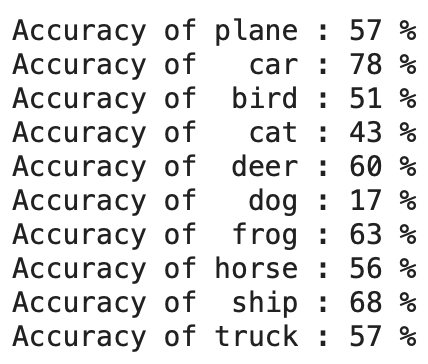
\includegraphics[width=1\linewidth]{images/q9_5.png}
      \caption{SGD optimizer}
      \label{fig:sub1}
    \end{subfigure}%
    \begin{subfigure}{.244\textwidth}
      \centering
      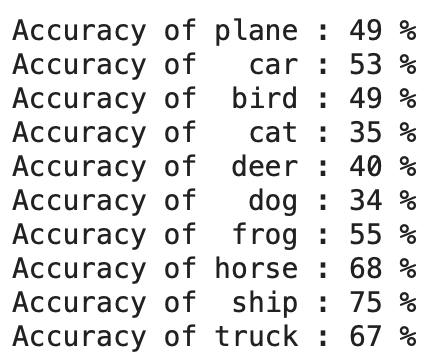
\includegraphics[width=1\linewidth]{images/q9_6.png}
      \caption{adam optimizer}
      \label{fig:sub2}
    \end{subfigure}
    \begin{subfigure}{.244\textwidth}
        \centering
        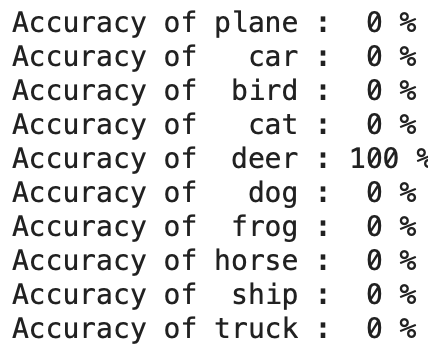
\includegraphics[width=1\linewidth]{images/q9_7.png}
        \caption{adam, lr=0.1}
        \label{fig:sub1}
      \end{subfigure}%
      \begin{subfigure}{.244\textwidth}
        \centering
        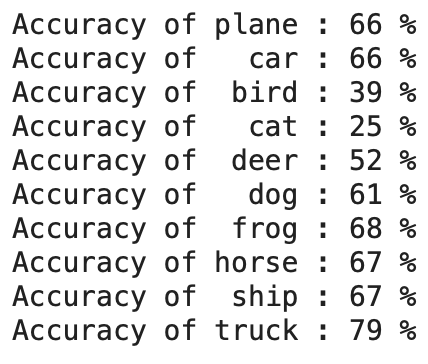
\includegraphics[width=1\linewidth]{images/q9_8.png}
        \caption{adam, 5 epochs}
        \label{fig:sub2}
      \end{subfigure}
    \caption{Performance of MLP build using pytorch}
    \label{fig:test}
\end{figure}

% SECTION
\section{Problem statement}
\textit{The impact on the performance of the network based on activation function change and adding new layers} 
\begin{itemize}
    \item Change in performance with relu
    \item Change in performance with adding layer 
    \item Change in performance with learning rate momentum
\end{itemize}

% SECTION
\section{Methodology}

\paragraph{Overview:}\textit{To accomplish the target problem solution, different training mechanism was used. Initially the training will was done with 60000 synthetic dataset. with this training data the network was trained in different stages by changing different parameters and observe the performance impact on the network.}

\paragraph{Strategy}\textit{The training script was build based on the given train\_mlp.py file. There are total four network was created to perform the testing. Initially the network was design with 2 layers and sigmoid as activation function of the hidden layer. Then new network with relu function was created. for this new network class MLP2 was created inside modules.py file and new class Relu was created in the ops.py file. Then for further testing a new MLP class was created with relu activation and three layers. Last but not least a simplified version of learning rate momentum was introduced by corelating the change with epochs}

\begin{itemize}
    \item Running the two layer neural network using relu activation function for the hidden layer.
    \item Change the activation function of hidden layer to relu function from sigmoid activation.
    \item Adding new layer on top of rule layer 
    \item Implementing momentum
\end{itemize}

% SECTION
\section{Experiments}
\paragraph{2 Layer Sigmoid}\textit{60000 intense of synthetic dataset was loaded and fed in the network. Total 20 epochs where used for the training where batch size was kept to 128 and the learning rate was 0.001}

\paragraph{2 Layer Relu}\textit{The next training was done on same dataset and parameters. However the new network of 2 layers was build where relu activation function was used to verify the performance.}

\paragraph{3 Layer Relu}\textit{Similar to above experiment all the parameters were kept same. However a new MLP was build with three layers where relu activation was used for hidden layer.}

\paragraph{Momentum}\textit{To experiment the performance of the network over momentum two layer network with relu activation was used. for this the learning rate was modified with the change of epochs}


% SECTION
\section{Results and discussion}

\paragraph{2 Layer Sigmoid}\textit{2 layers MLP with Sigmoid function has been considered here as the benchmark. From the figure 1 we can notice that for long time there was no improvement in training loss or accuracy, however after 13 epochs we can the the rapid improvement in both training loss and validation accuracy. This implies that this network may fall in to local optimum and may take time to recover. Overall performance of the system is worst than relu function.}

\paragraph{2 Layer Relu}\textit{Adding the relu activation function function in the hidden layer improved both training loss and validation accuracy. we can observe the validation accuracy quickly reaches close to 98 percent }

\paragraph{3 Layer Relu}\textit{Adding a new layer did not significantly improved the performance of the network from two layer relu activation. From the figure 1 we can see that it perform similar to 2 layer relu network. Considering the provided data is not significantly complex, we can conclude that 3 layers network is not required.}

\paragraph{Momentum}\textit{The performance of the momentum with respect to relu network is shown in the figure two. The simpler version of momentum change does not create any positive changes in performance. on the other hand we can see that network initially perform good similar to two layer relu then performance drastically drops.}

\begin{figure}[h!]
    \centering
    \begin{subfigure}{.5\textwidth}
      \centering
      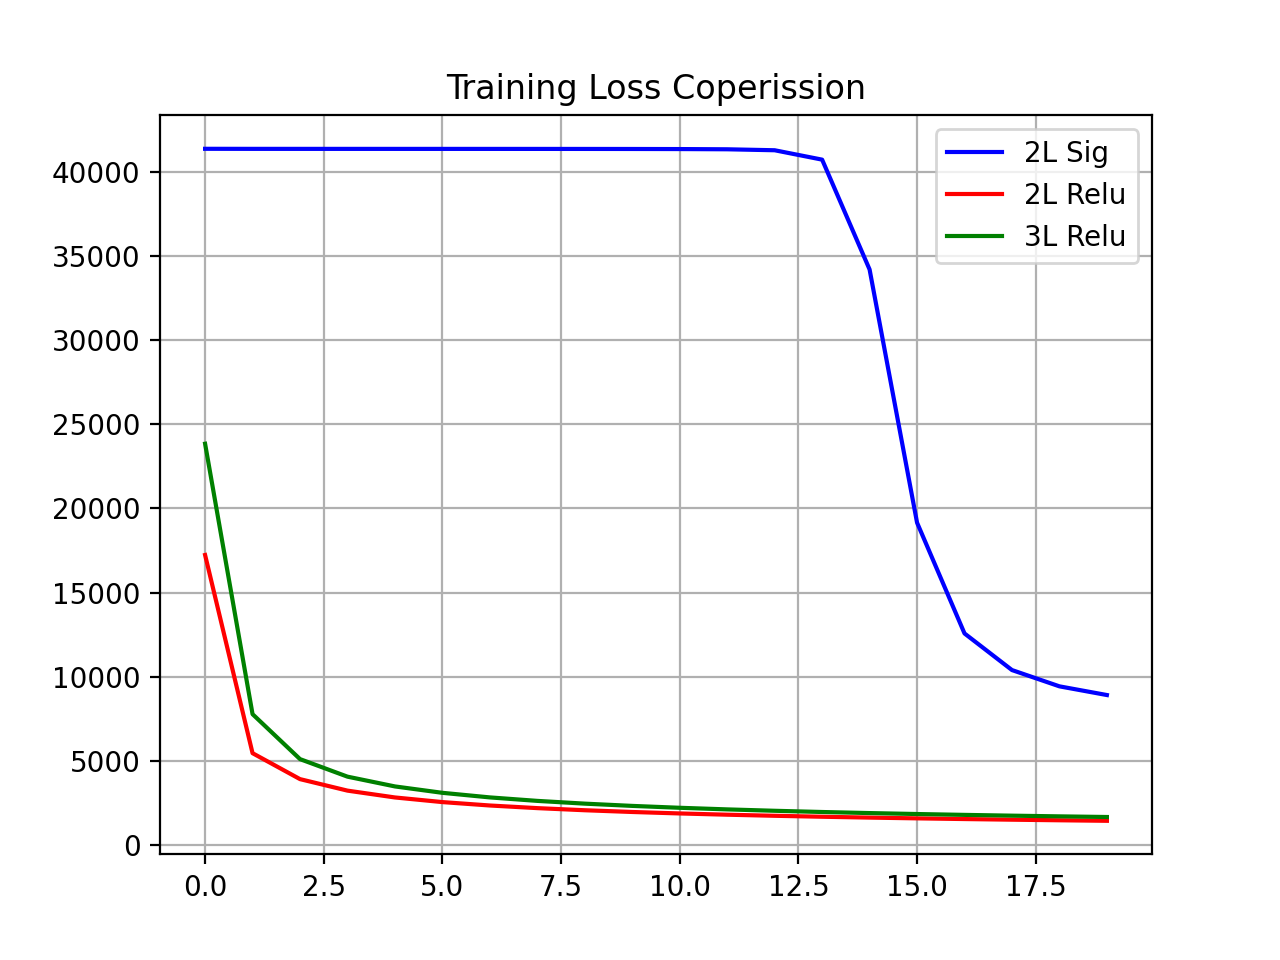
\includegraphics[width=.9\linewidth]{images/q9_1.png}
      \caption{Loss per epoch}
      \label{fig:sub1}
    \end{subfigure}%
    \begin{subfigure}{.5\textwidth}
      \centering
      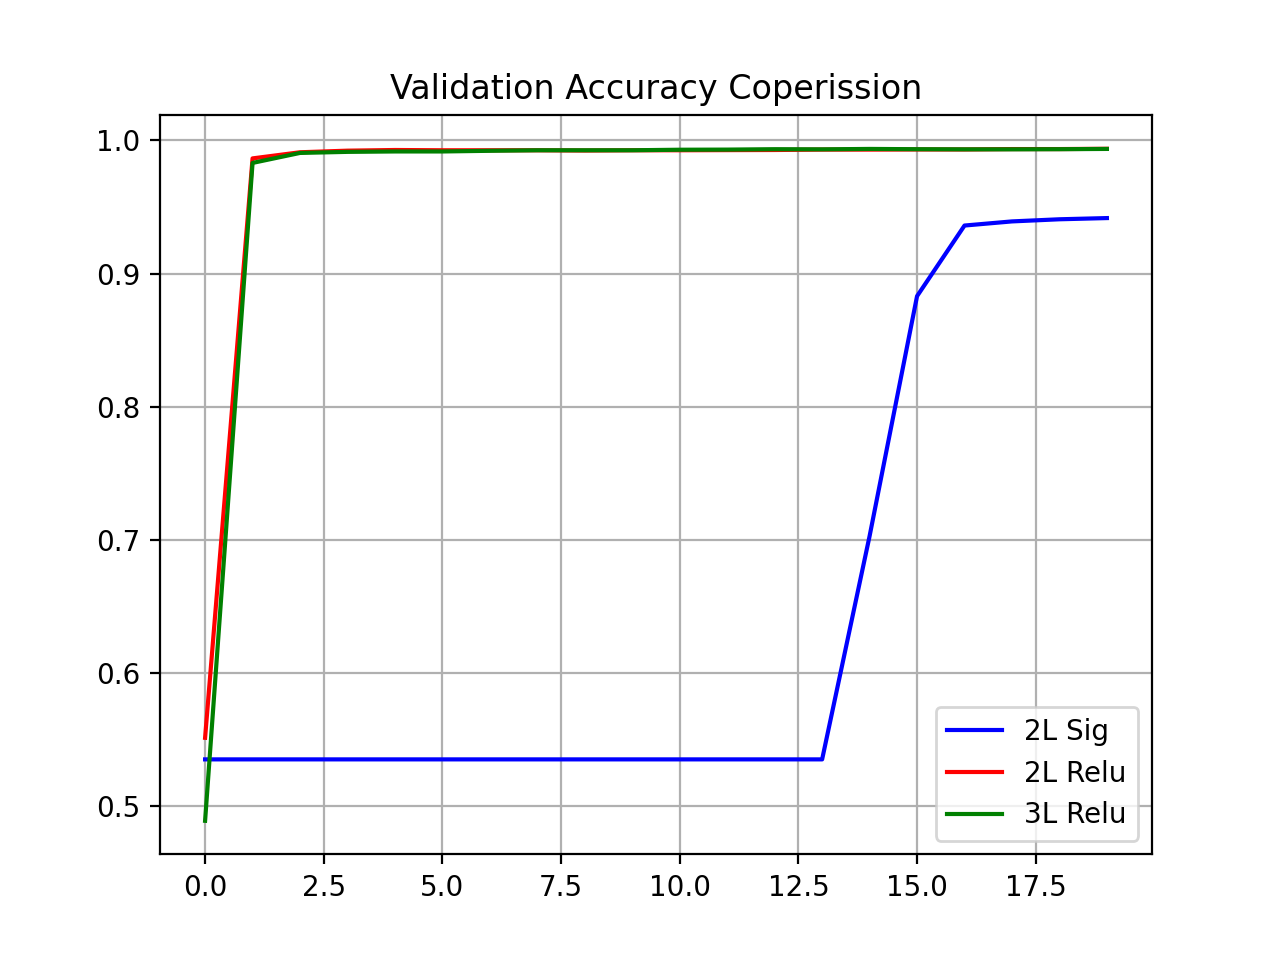
\includegraphics[width=.9\linewidth]{images/q9_2.png}
      \caption{Accuracy epochs}
      \label{fig:sub2}
    \end{subfigure}
    \caption{Loss and Accuracy over 20 epochs }
    \label{fig:test}
\end{figure}

\begin{figure}[h!]
    \centering
    \begin{subfigure}{.5\textwidth}
      \centering
      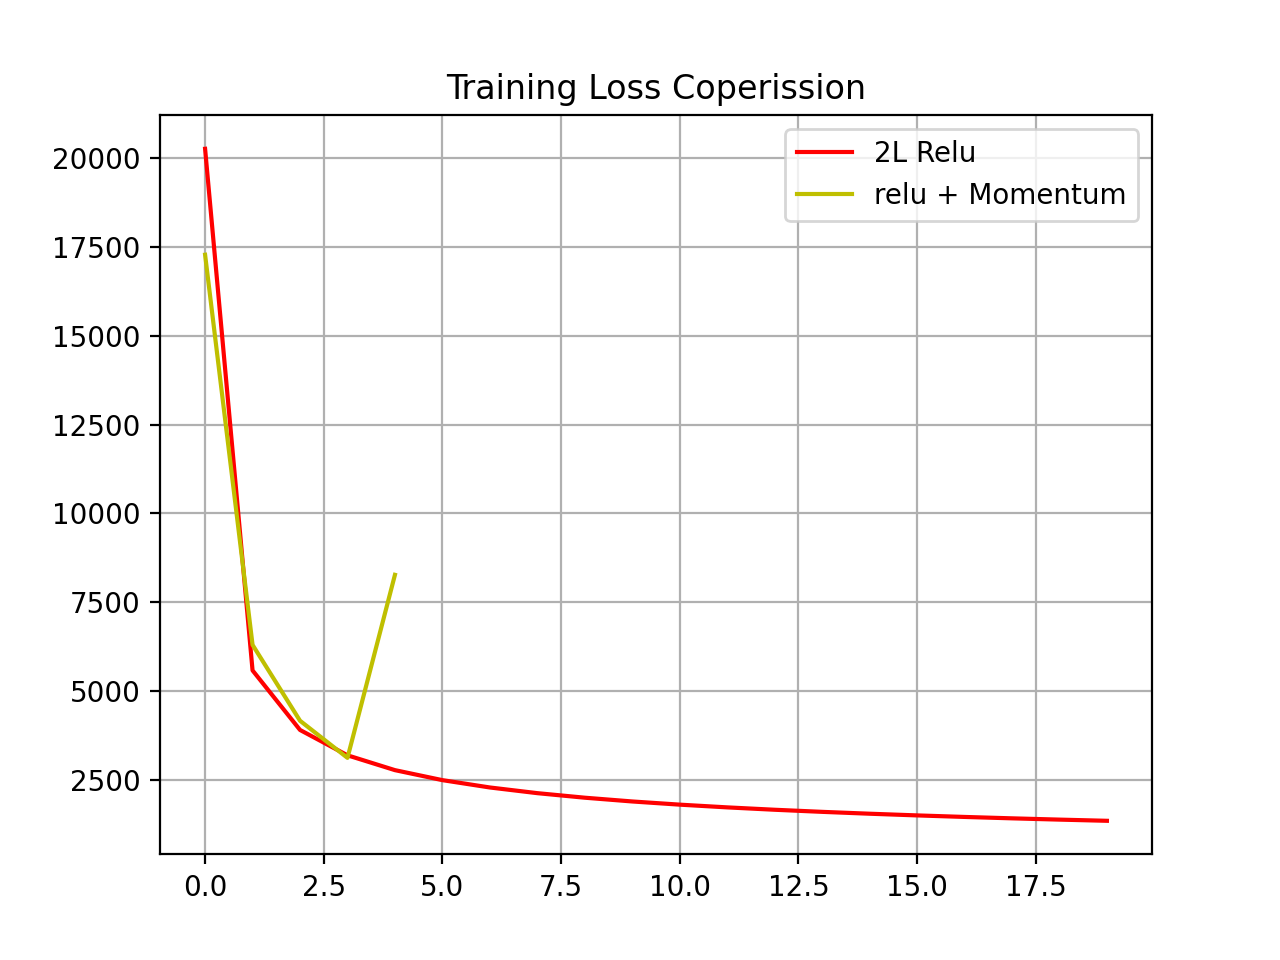
\includegraphics[width=.9\linewidth]{images/q9_3.png}
      \caption{Loss per epoch}
      \label{fig:sub1}
    \end{subfigure}%
    \begin{subfigure}{.5\textwidth}
      \centering
      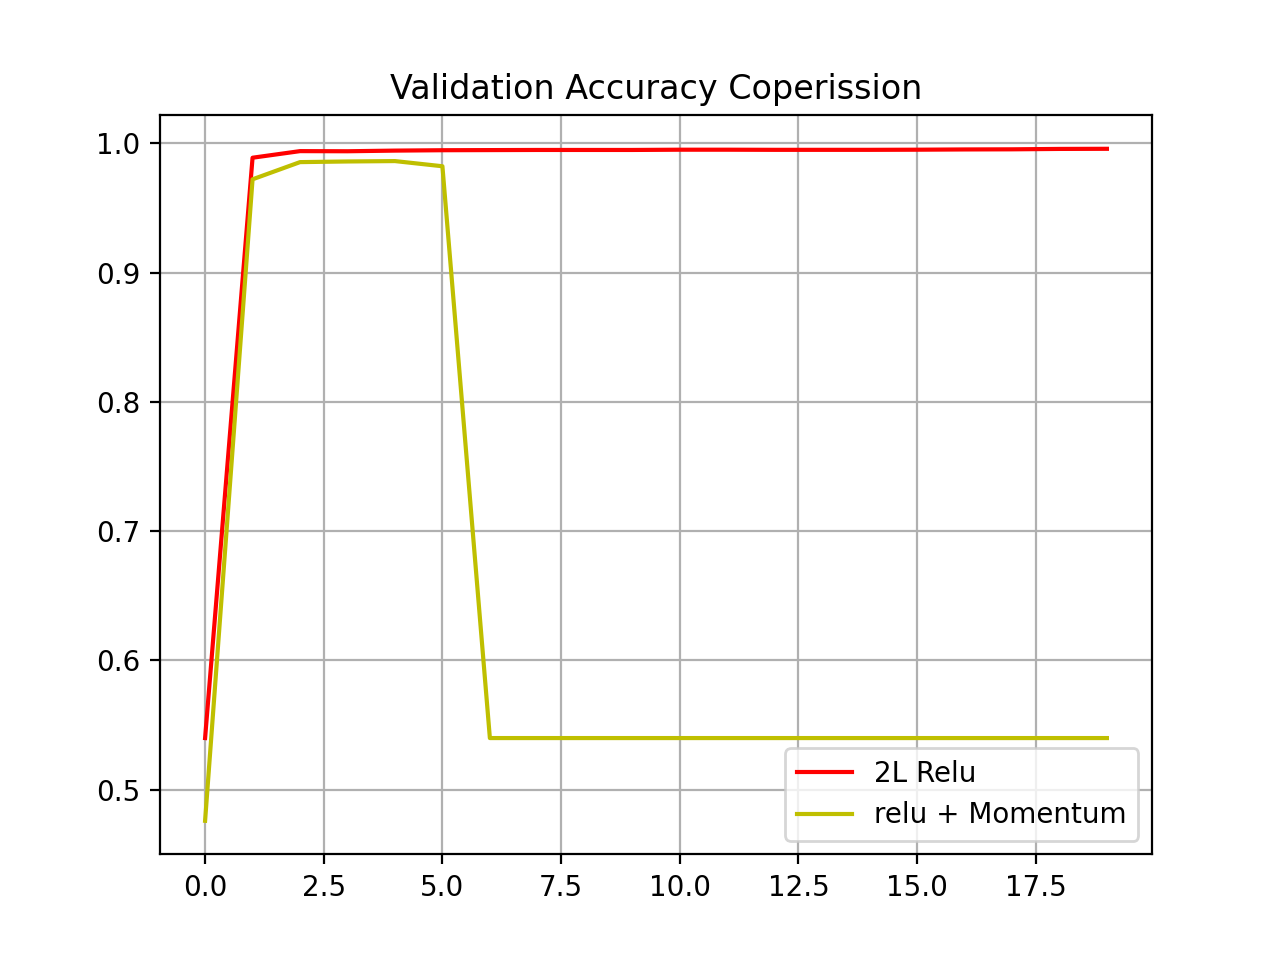
\includegraphics[width=.9\linewidth]{images/q9_4.png}
      \caption{Accuracy epochs}
      \label{fig:sub2}
    \end{subfigure}
    \caption{Loss and Accuracy for Momentum }
    \label{fig:test}
\end{figure}

% SECTION
\newpage
\section{A code snippet}
\paragraph{Relu Actiovation}\textit{}
\begin{lstlisting}[language=Python]
class Relu(Op):
    @staticmethod
    def forward(context, input):
        relux = np.maximum(0, input)
        context['input'] = input 
        return relux 
    @staticmethod
    def backward(context, goutput):
        g_in = goutput.copy()
        g_in[context['input'] <=0 ] = 0
        return g_in
\end{lstlisting}

\paragraph{3 Layer MLP}\textit{}
\begin{lstlisting}[language=Python]
class MLP3L(Module):
    def __init__(self, input_size, output_size, hidden_mult=2):
        super().__init__()
        hidden_size = hidden_mult * input_size
        self.layer1 = Linear(input_size, hidden_size)
        self.layer2 = Linear(hidden_size, hidden_size)
        self.layer3 = Linear(hidden_size, output_size)

    def forward(self, input):
        assert len(input.size()) == 2
        x = self.layer1(input)
        x = relu(x)
        x = self.layer2(x)
        x = relu(x)
        x = self.layer3(x)
        x = softmax(x)
        return x

    def parameters(self):
        return self.layer1.parameters() + self.layer2.parameters()
\end{lstlisting}


% SECTION
\citep{eiben2003introduction}.

\renewcommand\bibliographytypesize{\small}
\bibliographystyle{apalike}
\bibliography{literature.bib}

\appendix
\section*{Appendix}

NA

\end{document} 
